% --- IMPORTS ---
\documentclass[leqno]{article}
\usepackage{graphicx}
\usepackage{dsfont}
\usepackage{mathtools}
\usepackage{amssymb}
\usepackage{amsmath}
\usepackage{amsthm}
\usepackage{float}
\usepackage{ragged2e}
\usepackage{tensor}
\usepackage{fancyhdr}
\usepackage{empheq}
\usepackage[most]{tcolorbox}
\usepackage{enumitem}
\usepackage{dirtytalk}
\usepackage{marginnote}
\usepackage{microtype}
\usepackage[
  a4paper,
  left=0.8in,
  right=1in,
  top=1in,
  bottom=0.5in,
  headheight=14pt,
  headsep=0.4in
]{geometry}
\setlength{\parindent}{0cm}
% --- TikZ Packages ---
\usepackage{pgfplots}
\pgfplotsset{compat=1.18}
\usepgfplotslibrary{fillbetween, polar}
\usetikzlibrary{calc, positioning}
\usetikzlibrary{angles, quotes}
\usetikzlibrary{arrows.meta}
\usetikzlibrary{decorations.pathreplacing, decorations.markings}
\usetikzlibrary{patterns}
\usetikzlibrary{intersections}
% --- URL Packages ---
\usepackage[colorlinks=true,linkcolor=red,citecolor=magenta,urlcolor=black]{hyperref}%
\urlstyle{same}
% --- END OF IMPORTS ---

% --- CUSTOM COMMANDS ---
\RenewDocumentCommand{\marks}{o m}{%
  \IfValueTF{#1}%
    {\marginnote{\raggedright\textbf{[#2]}}[#1]}%
    {\marginnote{\raggedright\textbf{[#2]}}}%
}
\newcommand{\vspacerule}[2]{%
  \par\vspace*{#1}%
  \noindent\hrulefill\par
  \vspace*{#2}%
}
\definecolor{scarlet}{RGB}{205, 40, 75}
\newcommand{\questionitem}{%
  \item\phantomsection
  \addcontentsline{toc}{section}{Question \number\value{enumi}}%
}
\renewcommand{\contentsname}{Questions}
% --- END OF CUSTOM COMMANDS ---

% --- HEADER CONFIG ---
\pagestyle{fancy}
\fancyhead{}
\fancyfoot{}
\renewcommand{\headrulewidth}{0.9pt}
\lhead{Systems of Differential Equations}
\chead{}
\rhead{\href{https://danieljsmith.org}{danieljsmith.org}}
% --- END OF HEADER CONFIG ---

\begin{document}
\vspace*{20pt}
\tableofcontents
\newpage
\begin{enumerate}[
  label=\textbf{\arabic*.},
  leftmargin=*,
  topsep=0pt,
  partopsep=0pt,
  parsep=0pt
]

% ---- Question 1 ----
\questionitem

The functions $x$ and $y$ satisfy
\begin{align*}
\frac{\mathrm{d}x}{\mathrm{d}t}+\,\,\,y&=5x\\[5pt]
\frac{\mathrm{d}y}{\mathrm{d}t}+2y&=6x
\end{align*} \\
\begin{enumerate}[label=\textbf{(\alph*)}]
  \item Differentiate the first equation and eliminate $y$ to show that $x$ satisfies\\
  \[
  \frac{\mathrm{d}^2 x}{\mathrm{d}t^2}-3\frac{\mathrm{d}x}{\mathrm{d}t}-4x=0
  \]
  \marks[-30pt]{4}
  \item Given that $x=1$ and $y=3$ when $t=0$, find explicit expressions for $x$ and $y$ in terms of $t$. \marks{7} \\
\end{enumerate}

\newpage

% ---- Question 2 ----
\questionitem

The functions $x$ and $y$ satisfy the simultaneous differential equations \\
\begin{align*}
\frac{\mathrm{d}x}{\mathrm{d}t}+y&=0\\[5pt]
\frac{\mathrm{d}y}{\mathrm{d}t}-x&=2e^{t}
\end{align*}
and when $t=0$, $x=0$ and $y=1$. \\

Solve the system, giving $x$ and $y$ explicitly in terms of $t$ \marks{11} \\

\newpage

% ---- Question 3 ----
\questionitem

The functions $x$ and $y$ satisfy \\
\[
\begin{aligned}
\frac{\mathrm{d}x}{\mathrm{d}t} &= 3x+4y+7 \\[5pt]
\frac{\mathrm{d}y}{\mathrm{d}t} &= -x-y-1
\end{aligned}
\] \\

Given that $x=5$ and $y=-3$ when $t=0$, find $x$ and $y$ as functions of $t$ \marks{10} \\

\newpage

% ---- Question 4 ----
\questionitem

The functions $x$ and $y$ satisfy the system of differential equations
\begin{align*}
\frac{\mathrm{d}x}{\mathrm{d}t}&=x+2y-7 \\[5pt]
\frac{\mathrm{d}y}{\mathrm{d}t}&=2x+y-8
\end{align*}\\
\begin{enumerate}[label=\textbf{(\alph*)}]
  \item Find the stationary point of the system.\\ That is, find the values of $x$ and $y$ such that $\frac{\mathrm{d}x}{\mathrm{d}t}=0$ and $\frac{\mathrm{d}y}{\mathrm{d}t}=0$ \marks{2} \\
  \item Given that $x=4$ and $y=0$ when $t=0$, find the particular solutions for $x$ and $y$ in terms of $t$ \marks{8} \\
\end{enumerate}

\newpage

% ---- Question 5 ----
\questionitem

For $t\ge 0$, the functions $x=f(t)$ and $y=g(t)$ satisfy the coupled first-order differential equations. \\
\begin{align*}
\frac{\mathrm{d}x}{\mathrm{d}t}&=2x-y \\[5pt]
\frac{\mathrm{d}y}{\mathrm{d}t}&=x+2y
\end{align*} \\
Given that $x=1$ and $y=2$ when $t=0$, determine exact simplified expressions for $f(t)$ and $g(t)$ \marks{10} \\

\newpage

% ---- Question 6 ----
\questionitem

The functions $x$ and $y$ satisfy the simultaneous differential equations \\
\begin{align*}
\frac{\mathrm{d}x}{\mathrm{d}t}+y&=0\\[5pt]
\frac{\mathrm{d}y}{\mathrm{d}t}-x&=2
\end{align*}
and when $t=\dfrac{\pi}{2}$, $x=1$ and $y=2$. \\

Solve the system, giving $x$ and $y$ explicitly in terms of $t$ \marks{11} \\

\newpage

% ---- Question 7 ----
\questionitem

An ecologist is studying the effect of introducing a population of weed-eating snails into a lake containing an invasive waterweed. During the first few months, a temporary pollutant also affects the snail population. \\

At time $t$ months, the amount of waterweed, $w$, and the number of snails, $s$, are modelled by the differential equations \\
\begin{align*}
\frac{\mathrm{d}w}{\mathrm{d}t}&=4w-s \\[5pt]
\frac{\mathrm{d}s}{\mathrm{d}t}&=6w-s-48e^{-t} \\
\end{align*}

\begin{enumerate}[label=\textbf{(\alph*)}]
  \item Show that
  \[\frac{\mathrm{d}^2 w}{\mathrm{d}t^2}-3\frac{\mathrm{d}w}{\mathrm{d}t}+2w=48e^{-t}\]
  \marks[-20pt]{3}
  \item Find a general solution for the amount of waterweed at time $t$ months \marks{6} \\
  \item Find a general solution for the number of snails at time $t$ months \marks{2} \\
\end{enumerate}
The model predicts that, at time $T$ months, the waterweed will have been eliminated. \\
Given that $w=30$ and $s=110$ when $t=0$ \\
\begin{enumerate}[label=\textbf{(\alph*)}, resume]
  \item Find the value of $T$, giving your answer to 3 decimal places \marks{6} \\
  \item Suggest one limitation of the model \marks{1} \\
\end{enumerate}

\newpage

% ---- Question 8 ----
\questionitem

At the start of 2021, a survey began of the number of mature trees and saplings in a managed woodland. \\

At time $t$ years after the survey began, the number of mature trees, $m$, and the number of saplings, $s$, are modelled by the differential equations \\
\begin{align*}
\frac{\mathrm{d}m}{\mathrm{d}t}&=\frac{1}{4}s \\[5pt]
\frac{\mathrm{d}s}{\mathrm{d}t}&=-\frac{1}{20}m-\frac{1}{10}s \\
\end{align*}

\begin{enumerate}[label=\textbf{(\alph*)}]
  \item Show that
  \[\frac{\mathrm{d}^2 s}{\mathrm{d}t^2}+\frac{1}{10}\frac{\mathrm{d}s}{\mathrm{d}t}+\frac{1}{80}s=0\]
  \marks[-20pt]{3}
  \item Find a general solution for the number of saplings in the woodland at time $t$ years \marks{4} \\
  \item Hence find a general solution for the number of mature trees in the woodland at time $t$ years \marks{3} \\
\end{enumerate}
At the start of 2021 there were $20$ mature trees and $20$ saplings. \\
\begin{enumerate}[label=\textbf{(\alph*)}, resume]
  \item \begin{enumerate}[label=(\roman*)]
    \item According to this model, find the first value of $t$ for which no saplings remain, and state the year.
    \item According to this model, how many mature trees are there at that time?
    \item Use your answers to parts (i) and (ii) to comment on the suitability of the model.
  \end{enumerate}
  \marks[-10pt]{7} 
\end{enumerate}

\newpage

% ---- Question 9 ----
\questionitem

\begin{figure}[H]
    \centering
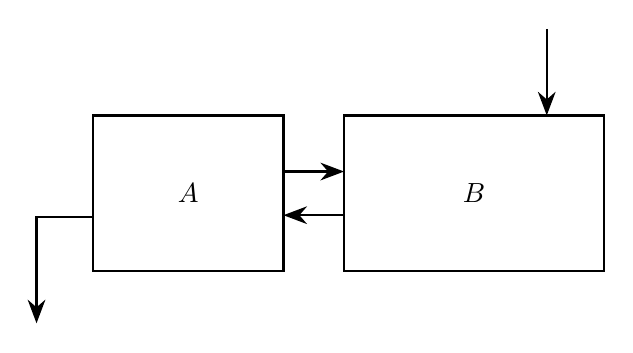
\begin{tikzpicture}[scale=1.1]
\def\aw{2.2}
\def\bw{3.0}
\def\th{1.8}
\def\gap{0.7}

\coordinate (A1) at (0,0);
\coordinate (A2) at (\aw,\th);
\coordinate (B1) at (\aw+\gap,0);
\coordinate (B2) at ({\aw+\gap+\bw},\th);

\draw[thick] (A1) rectangle (A2);
\draw[thick] (B1) rectangle (B2);

\node at ($(A1)!0.5!(A2)$) {$A$};
\node at ($(B1)!0.5!(B2)$) {$B$};

\coordinate (In1) at ({\aw+\gap+0.78*\bw},{\th+1});
\coordinate (In2) at ({\aw+\gap+0.78*\bw},\th);
\draw[thick,-{Stealth[length=3mm]}] (In1) -- (In2);

\coordinate (AB1) at (\aw,{0.64*\th});
\coordinate (AB2) at (\aw+\gap,{0.64*\th});
\draw[thick,-{Stealth[length=3mm]}] (AB1) -- (AB2);

\coordinate (BA1) at (\aw+\gap,{0.36*\th});
\coordinate (BA2) at (\aw,{0.36*\th});
\draw[thick,-{Stealth[length=3mm]}] (BA1) -- (BA2);

\coordinate (Out1) at (0,{0.35*\th});
\coordinate (Out2) at (-0.65,{0.35*\th});
\coordinate (Out3) at (-0.65,-0.6);
\draw[thick,-{Stealth[length=3mm]}] (Out1) -- (Out2) -- (Out3);
\end{tikzpicture}
\end{figure}

\vspace*{10pt}

A treatment system consists of two well-stirred tanks, $A$ and $B$. Tank $A$ has capacity 300 litres and tank $B$ has capacity 500 litres. \\

At time $t=0$, tank $A$ is full and contains 300 grams of salt, while tank $B$ is full and contains 1200 grams of salt. \\

When $t>0$, liquid flows in the following ways: \\
\begin{itemize}
  \item Brine with a salt concentration of $\mu$ grams per litre flows into tank $B$ at a constant rate
  \item Liquid flows from tank $A$ to tank $B$ at a rate of $3$ litres per minute
  \item Liquid flows from tank $B$ to tank $A$ at a rate of $r$ litres per minute
  \item Liquid flows out of tank $A$ through a waste pipe
  \item The amount of liquid in tank $A$ remains at $300$ litres and the amount of liquid in tank $B$ remains at $500$ litres \\
\end{itemize}
At time $t$ minutes ($t\ge 0$) there are $x$ grams of salt in tank $A$ and $y$ grams of salt in tank $B$. \\

This system is represented by the coupled differential equations

\begin{align*}
\dfrac{\mathrm{d}x}{\mathrm{d}t} & =  -\dfrac{1}{20}x+\dfrac{3}{100}y\\[6pt]
\dfrac{\mathrm{d}y}{\mathrm{d}t} & =  \dfrac{1}{100}x-\dfrac{3}{100}y + 24
\end{align*}
\\
\begin{enumerate}[label=\textbf{(\alph*)}]
  \item Find the value of $r$ \marks{2} \\
  \item Show that $\mu=2$ \marks{3} \\
  \item Solve the coupled differential equations to find both $x$ and $y$ in terms of $t$ \marks{9} \\
\end{enumerate}

\newpage

% ---- Question 10 ----
\questionitem

Two invasive plant species, $X$ and $Y$, are spreading through a wetland and compete for light and nutrients. A model for this competition assumes, in one particular wetland, the following. \\
\begin{itemize}
  \item In the absence of the other species, species $X$ would increase at a rate proportional to the number present, with constant of proportionality $p$.
  \item In the absence of the other species, species $Y$ would increase at a rate proportional to the number present, with constant of proportionality $q$.
  \item Competition reduces the rate of increase of species $X$ by an amount proportional to the number of species $Y$ present.
  \item Competition reduces the rate of increase of species $Y$ by an amount proportional to the number of species $X$ present. \\
\end{itemize}
If the numbers of species $X$ and $Y$ present at time $t$ years are $x$ and $y$ respectively, the model gives the differential equations 

\[\frac{\mathrm{d}x}{\mathrm{d}t}=px-ay \qquad \text{and} \qquad \frac{\mathrm{d}y}{\mathrm{d}t}=qy-bx\] \\
\begin{enumerate}[label=\textbf{(\alph*)}]
  \item 
  \begin{enumerate}[label=(\roman*)]
    \item Show that $x$ satisfies
    \[\frac{\mathrm{d}^2 x}{\mathrm{d}t^2}-(p+q)\frac{\mathrm{d}x}{\mathrm{d}t}+(pq-ab)x=0\]
    and hence that the general solution for $x$ is
    \[x=Ae^{\lambda_1 t}+Be^{\lambda_2 t}\]
    where $\lambda_1$ and $\lambda_2$ are the roots of
    \[\lambda^2-(p+q)\lambda+(pq-ab)=0\]
    \marks[-20pt]{6}
    \item Hence show that the general solution for $y$ can be written in the form
    \[y=\frac{p-\lambda_1}{a}Ae^{\lambda_1 t}+\frac{p-\lambda_2}{a}Be^{\lambda_2 t}\]
    \marks[-20pt]{2}
  \end{enumerate}
\end{enumerate}
Observations suggest that suitable values for the model are $p=0.035$, $q=0.005$, $a=0.03$ and $b=0.0225$. You should use these values in the rest of this question. \\
\begin{enumerate}[label=\textbf{(\alph*)}, resume]
  \item When $t=0$, the numbers present of species $X$ and $Y$ in this wetland are $x_0$ and $y_0$ respectively.
  \begin{enumerate}[label=(\roman*)]
    \item Show that
    \[x=\frac{1}{4}(3x_0-2y_0)e^{0.05t}+\frac{1}{4}(x_0+2y_0)e^{-0.01t}\]
    \marks[-20pt]{3}
    \item Hence show that
    \[y=-\frac{1}{8}(3x_0-2y_0)e^{0.05t}+\frac{3}{8}(x_0+2y_0)e^{-0.01t}\]
    \marks[-20pt]{1}
  \end{enumerate}
  \item Use initial values $x_0=400$ and $y_0=500$ with the results in part (b) to determine what the model predicts for each of the following. \\
  \begin{enumerate}[label=(\roman*)]
    \item What numbers of each species will be present after $25$ years? \marks{2} 
    \item When will the numbers of the two species be equal? \marks{4}
    \item Does either species ever disappear from the wetland? Justify your answer \marks{3} \\
  \end{enumerate}
  \item Different initial values will apply in other wetlands where the two species compete, but previous studies indicate that in most wetlands one population eventually increases while the other decreases.\\
  \begin{enumerate}[label=(\roman*)]
    \item Find a relation between $x_0$ and $y_0$ for which the model does not predict this outcome \marks{1} 
    \item Explain what the model predicts in the long term for this exceptional case \marks{2} 
  \end{enumerate}
\end{enumerate}

\newpage

% ---- Question 11 ----
\questionitem

A pharmacologist is studying the movement of a drug between a patient's bloodstream and muscle tissue. The amount of drug in the bloodstream after $t$ hours is $x$ mg. The amount of drug in the muscle tissue after $t$ hours is $y$ mg. Initially, when $t=0$, there is no drug in either the bloodstream or the muscle tissue. \\

At first it is assumed that no drug is removed from the body. The pharmacologist further assumes that the drug is infused into the bloodstream at a constant rate of $q$ mg per hour, where $q>6$. \\

For $t\ge 0$, this situation is modelled by the following pair of first-order linear differential equations. 

\begin{align*}
\frac{\mathrm{d}x}{\mathrm{d}t}&=-5x+30y+q \\[5pt]
\frac{\mathrm{d}y}{\mathrm{d}t}&=5x-30y
\end{align*} \\


\begin{enumerate}[label=\textbf{(\alph*)}]
  \item \begin{enumerate}[label=(\roman*)]
    \item Show that
    \[\frac{\mathrm{d}^2 x}{\mathrm{d}t^2}+35\frac{\mathrm{d}x}{\mathrm{d}t}=30q\]
    \marks[-20pt]{2}
    \item Hence determine $x$ in terms of $q$ and $t$ \marks{7} \\
    \item The patient's bloodstream is tested $20$ hours after the infusion begins. Explain why, according to this model, the patient will be at risk of toxic side effects when the test is carried out \marks{1} \\[10pt]
  \end{enumerate}
\end{enumerate}
Further observations suggest that some of the drug is metabolised in the muscle tissue and so is removed from the body. The model is refined in light of this. One resulting expression for $x$ is \\

\[x=q\left(10-e^{-17t}\left(10\cosh\!\left(\sqrt{241}\,t\right)+\frac{169}{\sqrt{241}}\sinh\!\left(\sqrt{241}\,t\right)\right)\right)\] \\

In the refined model, it is still assumed that the drug is infused at a constant rate. \\

\begin{enumerate}[label=\textbf{(\alph*)}, resume]
  \item Given now that $q<9$, determine whether the patient will be at risk of toxic side effects in the long run according to this refined model \marks{2} \\
  \item Suggest a reason why it might be more realistic to model the infusion rate as not being constant \marks{1} \\
\end{enumerate}

\newpage

% ---- Question 12 ----
\questionitem

A water-treatment plant uses two storage tanks, tank A and tank B, joined by a balancing pipe. At any given instant, water can be transferred between the two tanks. It is assumed that these transfers happen instantaneously. \\

The volume of water in tank A at time $t$ hours is denoted by $A$ and the corresponding volume in tank B is $B$. Because the volumes are large for most of the time, $A$ and $B$ are modelled as being continuous. \\

When the volumes in the two tanks are different, water is pumped from the tank with more water to the tank with less water. In addition, water flows directly into tank A at a rate proportional to $t^2$. An engineer therefore decides to model $A$ and $B$ with the following coupled differential equations. \\

\begin{align*}
\frac{\mathrm{d}A}{\mathrm{d}t}&=k(B-A)+\gamma t^2 \\
\frac{\mathrm{d}B}{\mathrm{d}t}&=k(A-B)
\end{align*} \\

\begin{enumerate}[label=\textbf{(\alph*)}]
  \item Explain why $k$ must be positive. \marks{1} \\
\end{enumerate}
After examining data, the engineer chooses $k=1$ and $\gamma=4$. \\
\begin{enumerate}[label=\textbf{(\alph*)}, resume]
  \item Show that $A$ satisfies the second order differential equation
  \[
  \frac{\mathrm{d}^2 A}{\mathrm{d}t^2}+2\frac{\mathrm{d}A}{\mathrm{d}t}=4t^2+8t
  \]
  \marks[-20pt]{2}
  \item
  \begin{enumerate}[label=(\roman*)]
    \item Find the complementary function for the differential equation from part (b). \marks{2}
    \item Explain why a particular integral of the form $A=at^2+bt+c$ will not work in this situation. \marks{1}
    \item Using a particular integral of the form $A=at^3+bt^2+ct$, find the general solution of the differential equation from part (b). \marks{3} \\
  \end{enumerate}
  \item At a certain time, tank A contains $52\,\mathrm{m^3}$ of water and the volume in tank A is increasing at $13\,\mathrm{m^3\,h^{-1}}$. Use the model, starting from this time, to estimate the volume of water in tank A $30$ minutes later. \marks{4} \\
  \item Explain why the model becomes unreliable as $t$ gets very large. \marks{1} \\
\end{enumerate}
\end{enumerate}
\end{document}
